\documentclass{beamer}
\usepackage{tikz}
\usepackage{pifont}
\usepackage{forest}
\usepackage{pgffor}
\usepackage{graphicx}
\graphicspath{ {./images/} }
% \usepackage{algorithm}
\usetikzlibrary{shapes}
% \usetheme{Madrid}
\usefonttheme{serif}

\let\oldemptyset\emptyset
\let\emptyset\varnothing

\newcommand{\xmark}{\ding{55}}%
\newcommand{\blank}{\underbar{\hphantom{aaaaaaaa}}}

\newcommand{\xbeginlgox}{\begin{minipage}{1in}\begin{tabbing}
  \quad\=\qquad\=\qquad\=\qquad\=\qquad\=\qquad\=\qquad\=\kill}
\newcommand{\xendlgox}{\end{tabbing}\end{minipage}}
\newenvironment{algorithm}{\begin{tabular}{|l|}\hline\xbeginlgox}
  {\xendlgox\\\hline\end{tabular}}


\begin{document}

\begin{frame}
  \frametitle{Graphs: Review}
  \begin{itemize}[<+->]
    \item (Abstract Def) An (undirected) \textcolor{blue}{graph} is a tuple $G = (V, E)$ where $V$ is any set and $E \subseteq \{\{u, v\} : u, v \in V\}$.
    \item (Usable Def) A graph is a set of vertices and edges between them.

    \begin{minipage}{0.4\linewidth}
      \begin{figure}
        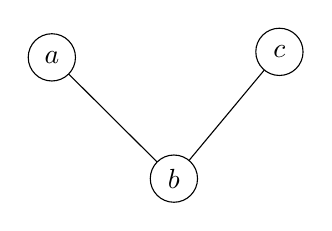
\begin{tikzpicture}[scale=0.1]
          \tikzstyle{every node}+=[inner sep=0pt]
          \draw [black] (24.3,-25.6) circle (3);
          \draw (24.3,-25.6) node {$a$};
          \draw [black] (39.8,-41) circle (3);
          \draw (39.8,-41) node {$b$};
          \draw [black] (53.2,-24.9) circle (3);
          \draw (53.2,-24.9) node {$c$};
          \draw [black] (26.43,-27.71) -- (37.67,-38.89);
          \draw [black] (41.72,-38.69) -- (51.28,-27.21);
        \end{tikzpicture}
        \caption{A graph with vertices $V = \{a, b, c\}$ and edges $E = \{\{a, b\}, \{b, c\}\}$.}
      \end{figure}
    \end{minipage} \hphantom{k} \vline \hphantom{k} \begin{minipage}{0.4\linewidth}
    \begin{figure}
      \begin{tikzpicture}[scale=0.1]
        \tikzstyle{every node}+=[inner sep=0pt]
        % \draw [black] (15.4,-10.4) circle (3);
        \draw (15.4,-10.4) node {$x$};
        % \draw [black] (27.7,-18.3) circle (3);
        \draw (27.7,-18.3) node {$2x - 5$};
        % \draw [black] (44.8,-10.4) circle (3);
        \draw (44.8,-10.4) node {$3x^2$};
        % \draw [black] (24.3,-36.1) circle (3);
        \draw (24.3,-36.1) node {$1$};
        % \draw [black] (63.2,-10.4) circle (3);
        \draw (63.2,-10.4) node {$x^2 + 4$};
        % \draw [black] (56.1,-22.8) circle (3);
        \draw (56.1,-22.8) node {$\frac{1}{2}x^2$};
        % \draw [black] (34.3,-46.1) circle (3);
        \draw (34.3,-46.1) node {$5$};
        % \draw [black] (41.6,-34.1) circle (3);
        \draw (41.6,-34.1) node {$e$};
        \draw [black] (60.2,-10.4) -- (47.8,-10.4);
        \draw [black] (17.92,-12.02) -- (25.18,-16.68);
        \draw [black] (57.59,-20.2) -- (61.71,-13);
        \draw [black] (54.08,-20.58) -- (46.82,-12.62);
        \draw [black] (35.86,-43.54) -- (40.04,-36.66);
        \draw [black] (38.62,-34.44) -- (27.28,-35.76);
        \draw [black] (26.42,-38.22) -- (32.18,-43.98);
        \end{tikzpicture}
        \caption{A graph with edges if nodes are Big-Theta of each other}
    \end{figure}
  \end{minipage}
\end{itemize}
\end{frame}

\begin{frame}
  \frametitle{Special Graphs}
  \begin{itemize}[<+->]
    \item The graph $K_n$ has $n$ nodes and an edge between every pair of vertices:
    \begin{figure}
      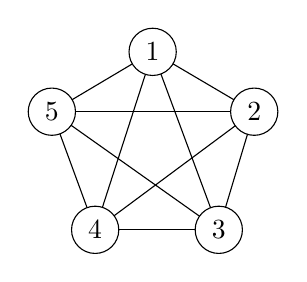
\begin{tikzpicture}[scale=0.1]
        \tikzstyle{every node}+=[inner sep=0pt]
        \draw [black] (36.6,-12.4) circle (3);
        \draw (36.6,-12.4) node {$1$};
        \draw [black] (49.5,-20) circle (3);
        \draw (49.5,-20) node {$2$};
        \draw [black] (45,-35) circle (3);
        \draw (45,-35) node {$3$};
        \draw [black] (29.3,-35) circle (3);
        \draw (29.3,-35) node {$4$};
        \draw [black] (23.8,-20) circle (3);
        \draw (23.8,-20) node {$5$};
        \draw [black] (26.38,-18.47) -- (34.02,-13.93);
        \draw [black] (39.18,-13.92) -- (46.92,-18.48);
        \draw [black] (48.64,-22.87) -- (45.86,-32.13);
        \draw [black] (42,-35) -- (32.3,-35);
        \draw [black] (28.27,-32.18) -- (24.83,-22.82);
        \draw [black] (37.65,-15.21) -- (43.95,-32.19);
        \draw [black] (35.68,-15.25) -- (30.22,-32.15);
        \draw [black] (46.5,-20) -- (26.8,-20);
        \draw [black] (42.55,-33.27) -- (26.25,-21.73);
        \draw [black] (31.71,-33.21) -- (47.09,-21.79);
        \end{tikzpicture}
        {$K_5$}
    \end{figure}
    \item The graph $C_n$ has $n$ nodes in a single cycle.
    \begin{figure}
      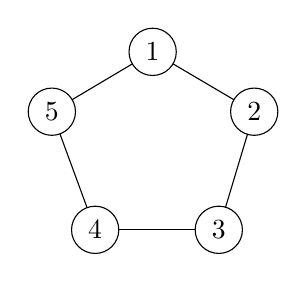
\begin{tikzpicture}[scale=0.1]
        \tikzstyle{every node}+=[inner sep=0pt]
        \draw [black] (36.6,-12.4) circle (3);
        \draw (36.6,-12.4) node {$1$};
        \draw [black] (49.5,-20) circle (3);
        \draw (49.5,-20) node {$2$};
        \draw [black] (45,-35) circle (3);
        \draw (45,-35) node {$3$};
        \draw [black] (29.3,-35) circle (3);
        \draw (29.3,-35) node {$4$};
        \draw [black] (23.8,-20) circle (3);
        \draw (23.8,-20) node {$5$};
        \draw [black] (26.38,-18.47) -- (34.02,-13.93);
        \draw [black] (39.18,-13.92) -- (46.92,-18.48);
        \draw [black] (48.64,-22.87) -- (45.86,-32.13);
        \draw [black] (42,-35) -- (32.3,-35);
        \draw [black] (28.27,-32.18) -- (24.83,-22.82);
      \end{tikzpicture}
      $C_5$
    \end{figure}
  \end{itemize}
\end{frame}

\begin{frame}
  \frametitle{Bipartite}
  A graph is \textcolor{blue}{bipartite} if its vertices can be divided into disjoint sets $L$ and $R$ such that every edge is between $L$ and $R$.
  
  \begin{center}
  
    **Bipartite $\Leftrightarrow$ 2-Colorable $\Leftrightarrow$ No odd cycles**
    \begin{minipage}{0.45\linewidth}
      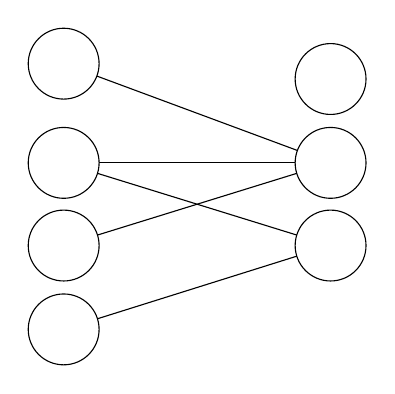
\begin{tikzpicture}[scale=0.15]
        \tikzstyle{every node}+=[inner sep=0pt]
        \draw [black] (23.1,-31.4) circle (3);
        \draw [black] (23.1,-24.3) circle (3);
        \draw [black] (23.1,-17.3) circle (3);
        \draw [black] (23.1,-8.9) circle (3);
        \draw [black] (45.7,-10.2) circle (3);
        \draw [black] (45.7,-17.3) circle (3);
        \draw [black] (45.7,-24.3) circle (3);
        \draw [black] (25.96,-30.5) -- (42.84,-25.2);
        \draw [black] (42.83,-18.19) -- (25.97,-23.41);
        \draw [black] (25.97,-18.19) -- (42.83,-23.41);
        \draw [black] (25.91,-9.95) -- (42.89,-16.25);
        \draw [black] (26.1,-17.3) -- (42.7,-17.3);
        \end{tikzpicture}
        \center{Bipartite}
    \end{minipage}\vline\hphantom{h}\begin{minipage}{0.45\linewidth}
      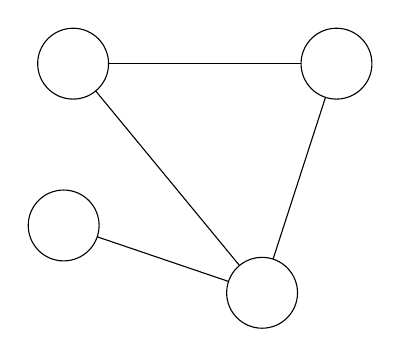
\begin{tikzpicture}[scale=0.15]
        \tikzstyle{every node}+=[inner sep=0pt]
        \draw [black] (40,-35.9) circle (3);
        \draw [black] (23.2,-30.2) circle (3);
        \draw [black] (24,-16.5) circle (3);
        \draw [black] (46.3,-16.5) circle (3);
        \draw [black] (40.93,-33.05) -- (45.37,-19.35);
        \draw [black] (27,-16.5) -- (43.3,-16.5);
        \draw [black] (37.16,-34.94) -- (26.04,-31.16);
        \draw [black] (38.09,-33.59) -- (25.91,-18.81);
        \end{tikzpicture}
        \center{Not bipartite}
    \end{minipage}
    
  \end{center}
\end{frame}

\begin{frame}
  \frametitle{Paths, Walks, and Cycles}
  A \textcolor{blue}{walk} in a graph is a sequence of vertices ($v_1, v_2, ..., v_k$) and edges ($e_1, e_2, ..., e_{k - 1}$) where each edge connects the two vertices on either end of it ($e_i = \{v_i, v_{i + 1}\}$).

  A \textcolor{blue}{path} is a walk that doesn't repeat vertices.

  A \textcolor{blue}{cycle} is a path where the start and end vertices are connected with an edge ($\{v_n, v_1\} \in E$).

  The \textcolor{blue}{distance} between two vertices is the length of the shortest path between them.

  \begin{center}
    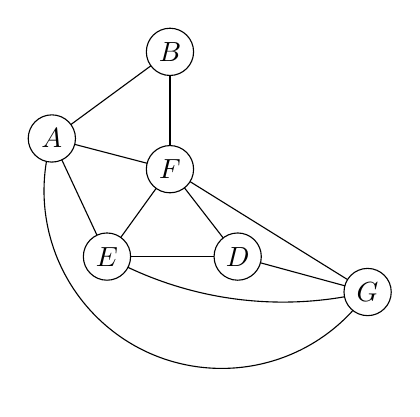
\begin{tikzpicture}[scale=0.1]
      \tikzstyle{every node}+=[inner sep=0pt]
      \draw [black] (21.2,-27.1) circle (3);
      \draw (21.2,-27.1) node {$F$};
      \draw [black] (21.2,-12.2) circle (3);
      \draw (21.2,-12.2) node {$B$};
      \draw [black] (6.2,-23.2) circle (3);
      \draw (6.2,-23.2) node {$A$};
      \draw [black] (13.2,-38.2) circle (3);
      \draw (13.2,-38.2) node {$E$};
      \draw [black] (29.8,-38.2) circle (3);
      \draw (29.8,-38.2) node {$D$};
      \draw [black] (46.3,-42.7) circle (3);
      \draw (46.3,-42.7) node {$G$};
      \draw [black] (19.45,-29.53) -- (14.95,-35.77);
      \draw [black] (23.04,-29.47) -- (27.96,-35.83);
      \draw [black] (21.2,-24.1) -- (21.2,-15.2);
      \draw [black] (18.3,-26.35) -- (9.1,-23.95);
      \draw [black] (18.78,-13.97) -- (8.62,-21.43);
      \draw [black] (7.47,-25.92) -- (11.93,-35.48);
      \draw [black] (16.2,-38.2) -- (26.8,-38.2);
      \draw [black] (43.41,-41.91) -- (32.69,-38.99);
      \draw [black] (43.75,-41.12) -- (23.75,-28.68);
      % \draw [black] (24.094,-12.987) arc (72.11203:6.79337:32.065);
      \draw [black] (44.432,-45.044) arc (-42.36557:-189.50028:22.561);
      \draw [black] (43.363,-43.307) arc (-80.18954:-115.29445:46.003);
      \end{tikzpicture}
  \end{center}
\end{frame}

\begin{frame}
  \frametitle{Connected Components}
  A \textcolor{blue}{connected component} of a graph is a maximal set of vertices where each pair has a connecting walk. The graph below can be split into 3 connected components.
  \begin{center}
    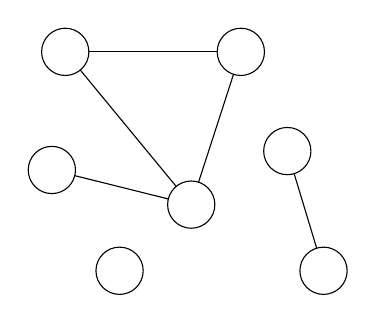
\begin{tikzpicture}[scale=0.1]
      \tikzstyle{every node}+=[inner sep=0pt]
      \draw [black] (40,-35.9) circle (3);
      \draw [black] (22.3,-31.5) circle (3);
      \draw [black] (24,-16.5) circle (3);
      \draw [black] (46.3,-16.5) circle (3);
      \draw [black] (52.2,-29.1) circle (3);
      \draw [black] (56.8,-44.3) circle (3);
      \draw [black] (30.9,-44.3) circle (3);
      \draw [black] (40.93,-33.05) -- (45.37,-19.35);
      \draw [black] (27,-16.5) -- (43.3,-16.5);
      \draw [black] (37.09,-35.18) -- (25.21,-32.22);
      \draw [black] (38.09,-33.59) -- (25.91,-18.81);
      \draw [black] (53.07,-31.97) -- (55.93,-41.43);
      \end{tikzpicture}
  \end{center}
\end{frame}

\begin{frame}
  \frametitle{Isomorphisms}
  \begin{itemize}[<+->]
    \item Two graphs $G = (V, E)$ and $G' = (V', E')$ are \textcolor{blue}{isomorphic} if there is a bijection $f: V \to V'$ such that $\{v_1, v_2\} \in E$ if and only if $\{f(v_1), f(v_2)\} \in E'$. (What type of relation is this?)
    
    \begin{center}
      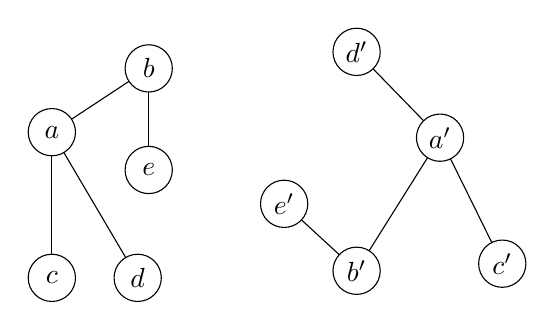
\begin{tikzpicture}[scale=0.1]
        \tikzstyle{every node}+=[inner sep=0pt]
        \draw [black] (23.2,-16.7) circle (3);
        \draw (23.2,-16.7) node {$b$};
        \draw [black] (23.2,-29.6) circle (3);
        \draw (23.2,-29.6) node {$e$};
        \draw [black] (21.8,-43.3) circle (3);
        \draw (21.8,-43.3) node {$d$};
        \draw [black] (10.9,-24.8) circle (3);
        \draw (10.9,-24.8) node {$a$};
        \draw [black] (10.9,-43.3) circle (3);
        \draw (10.9,-43.3) node {$c$};
        \draw [black] (49.6,-42.4) circle (3);
        \draw (49.6,-42.4) node {$b'$};
        \draw [black] (60.2,-25.5) circle (3);
        \draw (60.2,-25.5) node {$a'$};
        \draw [black] (40.4,-33.9) circle (3);
        \draw (40.4,-33.9) node {$e'$};
        \draw [black] (68.1,-41.5) circle (3);
        \draw (68.1,-41.5) node {$c'$};
        \draw [black] (49.6,-14.6) circle (3);
        \draw (49.6,-14.6) node {$d'$};
        \draw [black] (20.28,-40.72) -- (12.42,-27.38);
        \draw [black] (23.2,-26.6) -- (23.2,-19.7);
        \draw [black] (20.69,-18.35) -- (13.41,-23.15);
        \draw [black] (10.9,-40.3) -- (10.9,-27.8);
        \draw [black] (51.19,-39.86) -- (58.61,-28.04);
        \draw [black] (42.6,-35.94) -- (47.4,-40.36);
        \draw [black] (51.69,-16.75) -- (58.11,-23.35);
        \draw [black] (66.77,-38.81) -- (61.53,-28.19);
        \end{tikzpicture}
    \end{center}
  \end{itemize}
\end{frame}

\begin{frame}[t]
  \frametitle{Practice Questions I}
  \begin{itemize}[<+->]
    \item For which $n$ is $K_n$ bipartite? $C_n$?
    \item For a graph with $n$ vertices, what is an upper bound on the number of distinct paths?
    \item How many edges are in $K_n$? $C_n$?
    \item (SU24) Are these graphs isomorphic? What is the diameter of the left graph? What is the distance between $a$ and $c$?
    
    \begin{minipage}{0.49\linewidth}
      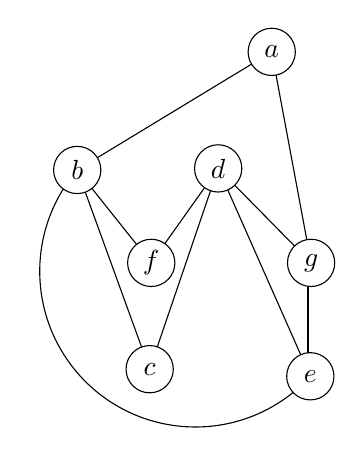
\begin{tikzpicture}[scale=0.1]
        \tikzstyle{every node}+=[inner sep=0pt]
        \draw [black] (6.4,-19.9) circle (3);
        \draw (6.4,-19.9) node {$b$};
        \draw [black] (24.3,-19.7) circle (3);
        \draw (24.3,-19.7) node {$d$};
        \draw [black] (31.1,-4.9) circle (3);
        \draw (31.1,-4.9) node {$a$};
        \draw [black] (15.8,-31.7) circle (3);
        \draw (15.8,-31.7) node {$f$};
        \draw [black] (36.1,-31.7) circle (3);
        \draw (36.1,-31.7) node {$g$};
        \draw [black] (36,-46.1) circle (3);
        \draw (36,-46.1) node {$e$};
        \draw [black] (15.6,-45.2) circle (3);
        \draw (15.6,-45.2) node {$c$};
        \draw [black] (8.27,-22.25) -- (13.93,-29.35);
        
        \draw [black] (17.53,-29.25) -- (22.57,-22.15);
        
        \draw [black] (7.43,-22.72) -- (14.57,-42.38);
        
        \draw [black] (16.57,-42.36) -- (23.33,-22.54);
        
        \draw [black] (34.78,-43.36) -- (25.52,-22.44);
        \draw [black] (35.7,-43.1) -- (35.7,-34.7);
        
        \draw [black] (34,-29.56) -- (26.4,-21.84);
        
        \draw [black] (35.55,-28.75) -- (31.65,-7.85);
        
        \draw [black] (8.96,-18.34) -- (28.54,-6.46);
        
        \draw [black] (33.817,-48.154) arc (-51.09452:-211.93182:19.767);
        
        \end{tikzpicture}
    \end{minipage}
    \begin{minipage}{0.49\linewidth}
      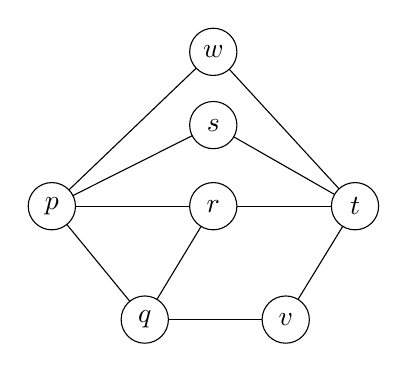
\begin{tikzpicture}[scale=0.1]
        \tikzstyle{every node}+=[inner sep=0pt]
        \draw [black] (49.1,-29.2) circle (3);
        \draw (49.1,-29.2) node {$t$};
        \draw [black] (10.6,-29.2) circle (3);
        \draw (10.6,-29.2) node {$p$};
        \draw [black] (40.3,-43.6) circle (3);
        \draw (40.3,-43.6) node {$v$};
        \draw [black] (31.1,-18.9) circle (3);
        \draw (31.1,-18.9) node {$s$};
        \draw [black] (22.4,-43.6) circle (3);
        \draw (22.4,-43.6) node {$q$};
        \draw [black] (31.1,-29.2) circle (3);
        \draw (31.1,-29.2) node {$r$};
        \draw [black] (31.1,-9.6) circle (3);
        \draw (31.1,-9.6) node {$w$};
        \draw [black] (46.5,-27.71) -- (33.7,-20.39);
        \draw [black] (28.42,-20.25) -- (13.28,-27.85);
        \draw [black] (47.07,-26.99) -- (33.13,-11.81);
        \draw [black] (28.93,-11.67) -- (12.77,-27.13);
        \draw [black] (28.1,-29.2) -- (13.6,-29.2);
        \draw [black] (20.5,-41.28) -- (12.5,-31.52);
        \draw [black] (25.4,-43.6) -- (37.3,-43.6);
        \draw [black] (47.54,-31.76) -- (41.86,-41.04);
        \draw [black] (46.1,-29.2) -- (34.1,-29.2);
        \draw [black] (23.95,-41.03) -- (29.55,-31.77);
        \end{tikzpicture}
    \end{minipage}
  \end{itemize}
\end{frame}

\begin{frame}
  \frametitle{Coloring}
  \begin{itemize}[<+->]
    \item A (proper) $k$-\textcolor{blue}{coloring} of a graph $G = (V, E)$ is an function $f: V \to \{1, 2, ..., k\}$ such that for every edge $\{u, v\} \in E, f(u) \neq f(v)$.
    \item The \textcolor{blue}{chromatic number} of a graph $G$ is $\chi(G)$, the smallest $k$ such that $G$ is $k$-colorable.
  \end{itemize}

  \begin{center}
    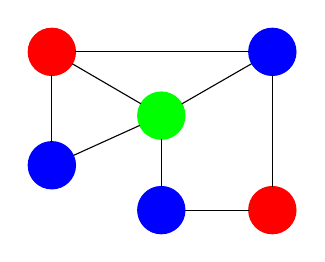
\begin{tikzpicture}[scale=0.1]
      \tikzstyle{every node}+=[inner sep=0pt]
      \draw [red, fill] (20.3,-16.1) circle (3);
      \draw [red, fill] (48.3,-36.2) circle (3);
      \draw [blue, fill] (48.3,-16.1) circle (3);
      \draw [blue, fill] (34.2,-36.2) circle (3);
      \draw [blue, fill] (20.3,-30.5) circle (3);
      \draw [green, fill] (34.2,-24.2) circle (3);
      \draw [black] (23.03,-29.26) -- (31.47,-25.44);
      \draw [black] (31.61,-22.69) -- (22.89,-17.61);
      \draw [black] (20.3,-19.1) -- (20.3,-27.5);
      \draw [black] (45.7,-17.59) -- (36.8,-22.71);
      \draw [black] (34.2,-33.2) -- (34.2,-27.2);
      \draw [black] (48.3,-33.2) -- (48.3,-19.1);
      \draw [black] (45.3,-36.2) -- (37.2,-36.2);
      \draw [black] (45.3,-16.1) -- (23.3,-16.1);
      \end{tikzpicture}
  \end{center}
  A 3-coloring of this graph (say, red means 1, blue means 2, and green means 3)
\end{frame}

\begin{frame}
  \frametitle{Coloring}
  \begin{itemize}[<+->]
    \item $K_n$ has an $n$-coloring, and no smaller number works.
    \item If $G$ has $K_n$ as a subgraph, $\chi(G) \geq n$.
    \item If $G$ can be colored with $k$ vertices, then $\chi(G) \leq k$.
  \end{itemize}
\end{frame}

\begin{frame}[t]
  \frametitle{Practice Questions II}
  \begin{itemize}[<+->]
    \item What is an upper bound for $\chi(G)$, given that $G$ has $n$ vertices?
    \item (SU24) What is the chromatic number of the graph below? Prove it.
    \begin{center}
      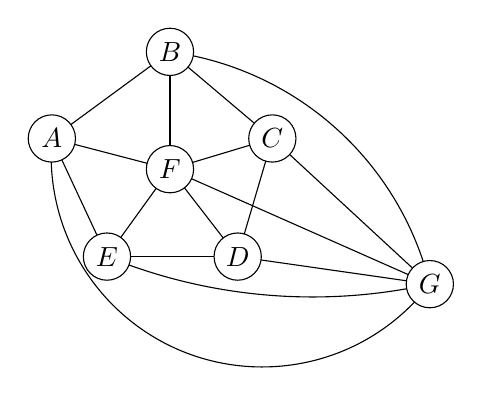
\begin{tikzpicture}[scale=0.1]
        \tikzstyle{every node}+=[inner sep=0pt]
        \draw [black] (21.2,-27.1) circle (3);
        \draw (21.2,-27.1) node {$F$};
        \draw [black] (21.2,-12.2) circle (3);
        \draw (21.2,-12.2) node {$B$};
        \draw [black] (6.2,-23.2) circle (3);
        \draw (6.2,-23.2) node {$A$};
        \draw [black] (13.2,-38.2) circle (3);
        \draw (13.2,-38.2) node {$E$};
        \draw [black] (29.8,-38.2) circle (3);
        \draw (29.8,-38.2) node {$D$};
        \draw [black] (34.2,-23.2) circle (3);
        \draw (34.2,-23.2) node {$C$};
        \draw [black] (54.2,-41.7) circle (3);
        \draw (54.2,-41.7) node {$G$};
        \draw [black] (19.45,-29.53) -- (14.95,-35.77);
        \draw [black] (23.04,-29.47) -- (27.96,-35.83);
        \draw [black] (24.07,-26.24) -- (31.33,-24.06);
        \draw [black] (21.2,-24.1) -- (21.2,-15.2);
        \draw [black] (18.3,-26.35) -- (9.1,-23.95);
        \draw [black] (18.78,-13.97) -- (8.62,-21.43);
        \draw [black] (7.47,-25.92) -- (11.93,-35.48);
        \draw [black] (16.2,-38.2) -- (26.8,-38.2);
        \draw [black] (30.64,-35.32) -- (33.36,-26.08);
        \draw [black] (31.91,-21.26) -- (23.49,-14.14);
        \draw [black] (52,-39.66) -- (36.4,-25.24);
        \draw [black] (51.23,-41.27) -- (32.77,-38.63);
        \draw [black] (51.46,-40.49) -- (23.94,-28.31);
        \draw [black] (24.156,-12.709) arc (78.03917:18.37126:39.375);
        \draw [black] (52.248,-43.976) arc (-43.83537:-178.31962:26.804);
        \draw [black] (51.258,-42.284) arc (-80.01954:-109.73901:68.989);
        \end{tikzpicture}
    \end{center}
  \end{itemize}
\end{frame}

\begin{frame}[t]
  \frametitle{Practice Questions II}
  \begin{itemize}[<+->]
    \item The \textit{degree} of a vertes is the number of edges incident to is. In a graph $G = (V, E)$, what is $\sum\limits_{v \in V} \deg(v)$?
    \item (Past Examlet) In a tree of height $h$, which best describes the diameter of the tree?\\
      (a) $h$
      (b) $2h$
      (c) $\leq 2h$
      (d) $h + 1$
      (e) $\leq h$
    % \item A \textit{planar} graph is a graph which can be drawn on a plane with no intersecting edges. Prove (by strong induction) Euler's theorem
    \begin{center}

    \end{center}
  \end{itemize}
\end{frame}

\begin{frame}[t]
  \frametitle{Tree Induction}
  Given a tree $T$ and a function $w: T \to \mathbb{R}_+$, the \textit{weighted sum} of the tree is $\sum\limits_{v \in T} w(v)2^{-h(v)}$, where $h(v)$ is the depth of the node.

  A weight function is \textit{fair} if, for every node $v \in T$,
  \begin{enumerate}
    \item If the node has one child $c$, $w(u) = w(c)$
    \item If the node has two children $c_1$ and $c_2$, $w(u) = w(c_1) + w(c_2)$
  \end{enumerate}
  Let $T$ be a tree and $r$ be its root. Prove by (strong) induction that for any fair weight function $w$, the weighed sum of the tree is no more than $2w(r)$.
\end{frame}

\begin{frame}
  \frametitle{Questions/Examples}
  \pause
  \pause
  \pause
\end{frame}

\end{document}